\documentclass[11pt]{article}

\usepackage[margin=1in]{geometry}
\usepackage{booktabs}
\usepackage{array}
\usepackage{hyperref}
\usepackage{caption}
\usepackage{float}
\usepackage{xcolor}
\usepackage{pgfplots}
\pgfplotsset{compat=1.18}

\hypersetup{
  colorlinks=true,
  linkcolor=blue,
  urlcolor=blue,
  citecolor=blue
}

\title{\textbf{Financial Disclosure Anomalies in Kerala Assembly Election Affidavits, 2016--2026}\\
\large An Open-Source Triage Note for Further Public-Interest Research}
\author{Kerala Election Financial Disclosure Project}
\date{May 2026}

\begin{document}
\maketitle

\begin{abstract}
This short paper studies candidate financial disclosures from Kerala Assembly elections in 2016, 2021, and 2026 using MyNeta/ADR affidavit data. It does not make findings of illegality. Instead, it builds a triage framework for identifying cases that merit deeper documentary verification. Across 2,900 candidate-election records, the analysis finds a sharp rise in declared median assets, an increase in high-triage records, and a subset of repeat candidates with unusually large asset growth or large income-to-asset gaps. The paper presents ranked investigative leads, party-level patterns, and a case vignette on P V Anvar to illustrate how affidavit anomalies can be connected with public proceedings and open research questions. The aim is to guide journalists, researchers, students, and civic technologists toward careful document-based inquiry.
\end{abstract}

\section{Introduction}

Election affidavits are one of the few structured public windows into the finances of political candidates. They are not full audits, but they allow longitudinal comparison of assets, liabilities, income disclosures, business interests, and criminal-case declarations. This paper uses those disclosures to ask a narrow research question: \emph{which candidate records show financial patterns that deserve further verification?}

The word ``anomaly'' is used deliberately. A high-asset candidate, a large loan, or a low declared income relative to assets is not by itself evidence of misconduct. Many candidates may have legitimate business income, inherited property, family assets, or lawful borrowing. The value of this analysis is prioritization: it helps identify where a document trail should be checked first.

\section{Data and Method}

The dataset contains 2,900 candidate-election records scraped from MyNeta/ADR pages for Kerala Assembly elections:

\begin{itemize}
  \item 2016: 1,112 candidate records;
  \item 2021: 925 candidate records;
  \item 2026: 863 candidate records.
\end{itemize}

The extraction pipeline collected candidate name, party, constituency, total assets, movable assets, immovable assets, liabilities, self and spouse income-tax-return income, PAN status, criminal-case count, and source URL. Repeat candidates were matched using normalized names, party/constituency hints, and fuzzy matching. A candidate-election suspicion score was then constructed from six categories:

\begin{enumerate}
  \item year-relative asset percentile;
  \item absolute asset thresholds;
  \item liabilities and debt-to-asset ratio;
  \item assets-to-declared-income ratio;
  \item criminal-case count;
  \item repeat-candidate asset growth and CAGR.
\end{enumerate}

Single-election candidates are still scored, but marked separately because no longitudinal growth pattern can be inferred. Repeat-candidate matches below high confidence require manual review before their growth metrics are used for any substantive claim.

\section{Aggregate Findings}

The declared asset distribution shifts upward across the three elections. Median declared assets rise from Rs 0.22 crore in 2016 to Rs 0.35 crore in 2021 and Rs 0.70 crore in 2026. The 90th percentile rises from Rs 1.84 crore to Rs 5.16 crore over the same period.

\begin{figure}[H]
\centering
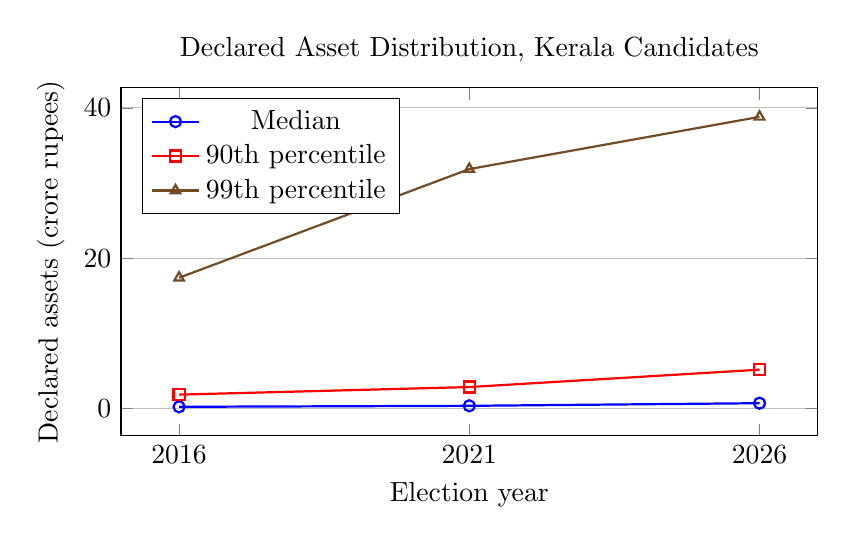
\begin{tikzpicture}
\begin{axis}[
    width=0.86\linewidth,
    height=6cm,
    xlabel={Election year},
    ylabel={Declared assets (crore rupees)},
    title={Declared Asset Distribution, Kerala Candidates},
    symbolic x coords={2016,2021,2026},
    xtick=data,
    ymajorgrids=true,
    legend pos=north west
]
\addplot+[mark=o, thick] coordinates {(2016,0.22) (2021,0.35) (2026,0.70)};
\addlegendentry{Median}

\addplot+[mark=square, thick] coordinates {(2016,1.84) (2021,2.85) (2026,5.16)};
\addlegendentry{90th percentile}

\addplot+[mark=triangle, thick] coordinates {(2016,17.40) (2021,31.86) (2026,38.81)};
\addlegendentry{99th percentile}
\end{axis}
\end{tikzpicture}
\caption{Declared asset distribution across Kerala candidate records.}
\end{figure}

The share of high-triage records also increases. Using a score threshold of 55, 18 records are flagged in 2016, 56 in 2021, and 71 in 2026. In percentage terms, this is approximately 1.6\%, 6.1\%, and 8.2\% of candidate-election records respectively.

\begin{figure}[H]
\centering
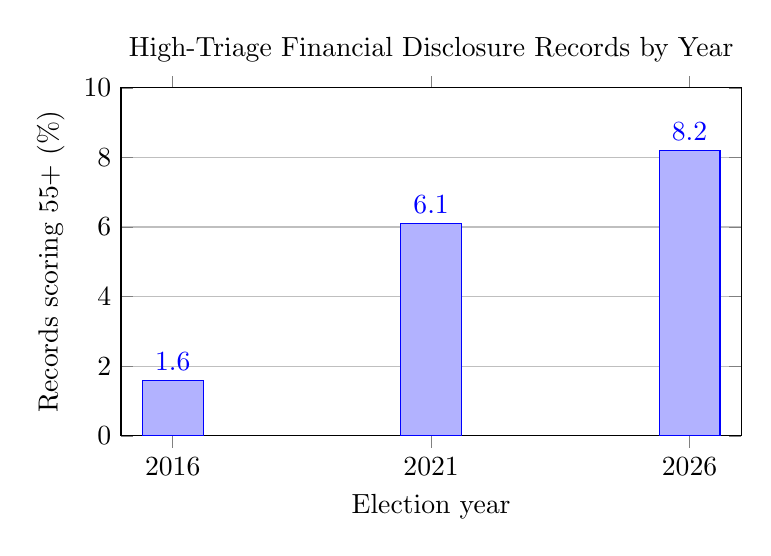
\begin{tikzpicture}
\begin{axis}[
    ybar,
    width=0.78\linewidth,
    height=6cm,
    symbolic x coords={2016,2021,2026},
    xtick=data,
    xlabel={Election year},
    ylabel={Records scoring 55+ (\%)},
    title={High-Triage Financial Disclosure Records by Year},
    nodes near coords,
    ymin=0,
    ymax=10,
    ymajorgrids=true,
    bar width=22pt
]
\addplot coordinates {(2016,1.6) (2021,6.1) (2026,8.2)};
\end{axis}
\end{tikzpicture}
\caption{Share of candidate-election records crossing the high-triage threshold.}
\end{figure}

Party-level patterns should be read carefully because candidate selection, incumbency, alliance structure, and local wealth distribution all affect candidate profiles. Among major/relevant parties, the number of high-triage records is largest for INC, BJP, CPI(M), IND, and IUML variants. Smaller parties can show high percentages because their denominators are small.

\begin{figure}[H]
\centering
\begin{tikzpicture}
\begin{axis}[
    xbar,
    width=0.9\linewidth,
    height=8cm,
    xlabel={Records scoring 55+ (\%)},
    symbolic y coords={CPI,Kerala Congress (M),CPI(M),IND,BJP,INC,IUML,Indian Union Muslim League},
    ytick=data,
    xmin=0,
    xmax=50,
    nodes near coords,
    xmajorgrids=true,
    title={High-Triage Share Among Major/Relevant Party Labels}
]
\addplot coordinates {
    (2.8,CPI)
    (10.5,Kerala Congress (M))
    (6.1,CPI(M))
    (1.5,IND)
    (6.5,BJP)
    (13.7,INC)
    (17.0,IUML)
    (44.0,Indian Union Muslim League)
};
\end{axis}
\end{tikzpicture}
\caption{High-triage share among major and analytically relevant party labels.}
\end{figure}

\section{Repeat Candidates}

Repeat candidates provide the strongest starting point for deeper work because their disclosures can be compared across time. The pipeline identified 583 repeat-candidate matches. Some candidates show large absolute asset growth, high compound annual growth rates, or large changes in liabilities. These patterns are leads, not conclusions: they require affidavit-level confirmation, inflation adjustment, family-asset review, and external records.

\begin{figure}[H]
\centering
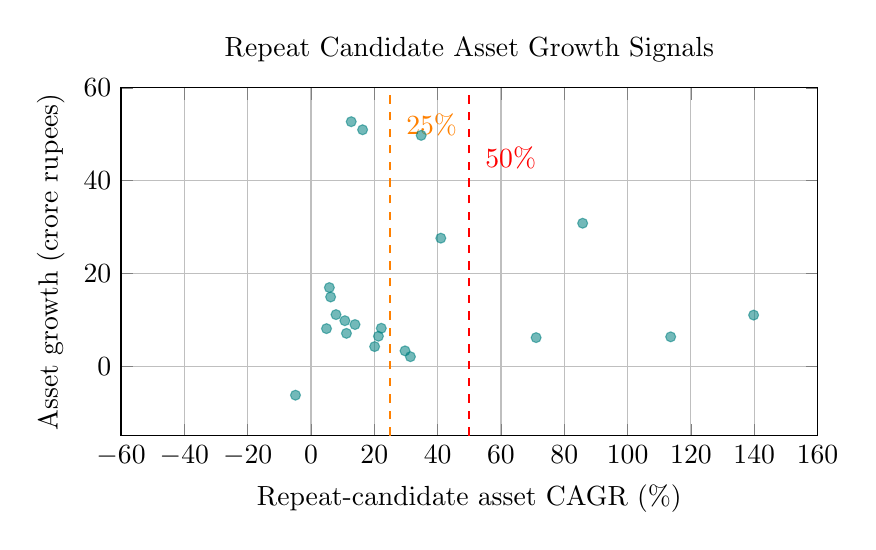
\begin{tikzpicture}
\begin{axis}[
    width=0.86\linewidth,
    height=6cm,
    xlabel={Repeat-candidate asset CAGR (\%)},
    ylabel={Asset growth (crore rupees)},
    title={Repeat Candidate Asset Growth Signals},
    grid=major,
    xmin=-60,
    xmax=160,
    ymin=-15,
    ymax=60,
    scatter/classes={
        a={mark=*,draw=teal,fill=teal}
    }
]
\addplot[scatter,only marks,scatter src=explicit symbolic,mark size=1.8pt,opacity=0.55]
coordinates {
    (12.7,52.71) [a]
    (16.3,50.97) [a]
    (34.8,49.76) [a]
    (85.8,30.82) [a]
    (41.0,27.60) [a]
    (5.8,16.95) [a]
    (6.2,14.92) [a]
    (7.9,11.12) [a]
    (139.8,11.02) [a]
    (10.7,9.81) [a]
    (13.9,8.98) [a]
    (22.2,8.18) [a]
    (4.9,8.10) [a]
    (11.2,7.08) [a]
    (21.3,6.46) [a]
    (71.1,6.16) [a]
    (113.6,6.33) [a]
    (20.1,4.23) [a]
    (29.7,3.31) [a]
    (31.4,2.05) [a]
    (-4.9,-6.25) [a]
};
\addplot[dashed, orange, thick] coordinates {(25,-15) (25,60)};
\addplot[dashed, red, thick] coordinates {(50,-15) (50,60)};
\node[anchor=west, orange] at (axis cs:27,52) {25\%};
\node[anchor=west, red] at (axis cs:52,45) {50\%};
\end{axis}
\end{tikzpicture}
\caption{Repeat-candidate asset growth and CAGR. Vertical lines mark 25\% and 50\% annualized growth.}
\end{figure}

\section{Top Triage Leads}

Table~\ref{tab:top} lists the top ten candidate-election records by the scoring model. These candidates should be treated as a manual-review queue. The reasons include high assets, liabilities, income-to-asset mismatch, criminal-case count, repeat growth, or a combination of these factors.

\begin{table}[H]
\centering
\small
\begin{tabular}{r l r l r r}
\toprule
Rank & Candidate & Year & Party & Assets (cr) & Score \\
\midrule
1 & P V Anvar S/o Shoukathali & 2026 & IND & 65.36 & 126.75 \\
2 & Vijay Hari & 2021 & INC & 32.28 & 124.95 \\
3 & P V Anvar & 2021 & IND & 64.15 & 119.26 \\
4 & Mani C Kappen & 2026 & IND & 21.68 & 109.06 \\
5 & V. Abdurahiman & 2026 & CPI(M) & 28.51 & 105.12 \\
6 & Shibu Baby John & 2026 & RSP & 24.63 & 104.57 \\
7 & Anoop Jacob & 2021 & Kerala Congress (Jacob) & 18.73 & 102.30 \\
8 & M P Joseph & 2021 & Kerala Congress & 11.16 & 101.10 \\
9 & Shibu Theckumpuram & 2026 & Kerala Congress & 68.65 & 95.94 \\
10 & Adv. Sangeetha Viswanadhan & 2026 & BDJS & 10.43 & 95.89 \\
\bottomrule
\end{tabular}
\caption{Top candidate-election triage records. Scores are prioritization signals, not findings.}
\label{tab:top}
\end{table}

\section{Case Vignette: P V Anvar}

P V Anvar illustrates why the method combines multiple signals rather than simply ranking by income or assets. He is not the highest-income candidate in the dataset. His record is prioritized because of a combination of declared asset growth, high liabilities, income-to-asset mismatch, criminal-case count, and public allegations concerning related business entities and loans.

His declared assets rise from Rs 14.39 crore in 2016 to Rs 64.15 crore in 2021, an increase of about Rs 49.76 crore. By 2026, assets remain near Rs 65.36 crore, while liabilities rise to Rs 40.07 crore. Public sources, including an Enforcement Directorate press release, discuss allegations involving Kerala Financial Corporation loans, PVR Metro Village LLP, Peeveeaar Developers Pvt Ltd, collateral, possible benami holdings, and a Sierra Leone-linked angle. These public allegations do not prove misconduct, but they create clear verification tasks: compare affidavit liabilities with loan documents, MCA filings, collateral records, land records, and any foreign registry entries.

\begin{figure}[H]
\centering
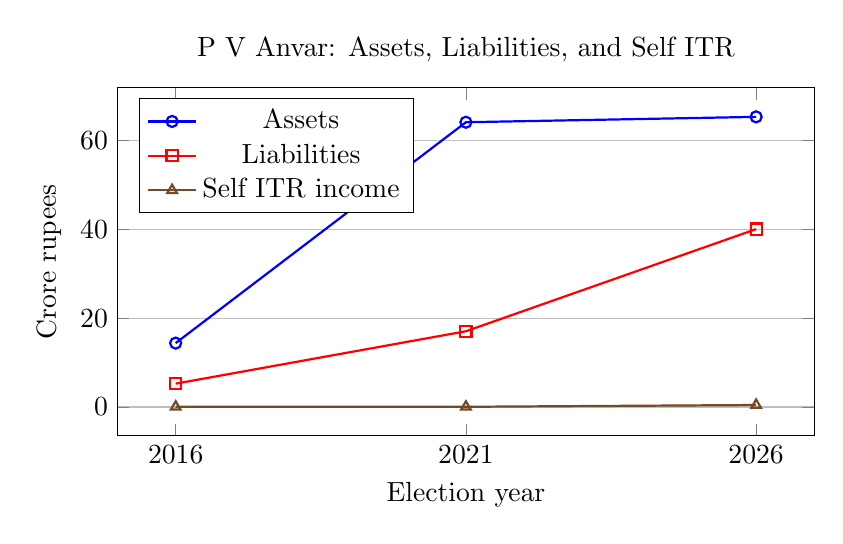
\begin{tikzpicture}
\begin{axis}[
    width=0.86\linewidth,
    height=6cm,
    xlabel={Election year},
    ylabel={Crore rupees},
    title={P V Anvar: Assets, Liabilities, and Self ITR},
    symbolic x coords={2016,2021,2026},
    xtick=data,
    ymajorgrids=true,
    legend pos=north west
]
\addplot+[mark=o, thick] coordinates {(2016,14.39) (2021,64.15) (2026,65.36)};
\addlegendentry{Assets}

\addplot+[mark=square, thick] coordinates {(2016,5.25) (2021,17.06) (2026,40.07)};
\addlegendentry{Liabilities}

\addplot+[mark=triangle, thick] coordinates {(2016,0.046) (2021,0.040) (2026,0.438)};
\addlegendentry{Self ITR income}
\end{axis}
\end{tikzpicture}
\caption{P V Anvar's declared assets, liabilities, and self ITR income.}
\end{figure}

\section{Future Work}

This project should be extended in five directions:

\begin{enumerate}
  \item \textbf{Affidavit audit packs:} create a top-100 review pack with source URLs, raw tables, and manual verification fields.
  \item \textbf{Family asset movement:} parse self, spouse, HUF, and dependent asset totals separately across years.
  \item \textbf{Company and charge records:} connect candidate names and disclosed companies to MCA filings, LLP partners, directors, charges, and loan collateral.
  \item \textbf{Land and procurement linkage:} compare immovable-property schedules with land-board orders, local body permits, environmental proceedings, and government contract data.
  \item \textbf{Case classification:} separate political/protest criminal cases from financial, property, environmental, and violence-related cases.
\end{enumerate}

The most promising research direction is not to accuse from a spreadsheet, but to build document trails. A reproducible workflow can help curious citizens and researchers ask better questions: which assets grew, whose assets grew, what loans financed them, what entities held them, and whether the disclosures align with public records.

\section{Conclusion}

Kerala candidate affidavit data reveal rising declared assets, increasing high-triage financial disclosure records, and a meaningful set of repeat candidates whose asset growth or liability patterns deserve closer review. The findings are best understood as a map of open questions. For public-interest research, the next step is to combine affidavit data with court records, company filings, land records, loan charge documents, and foreign registry checks. That is where disclosure anomalies can become evidence-backed stories, or be resolved as lawful and explainable financial activity.

\section*{References}

\begin{itemize}
  \item MyNeta/ADR candidate affidavit pages for Kerala Assembly elections, 2016, 2021, and 2026.
  \item Enforcement Directorate press release on P V Anvar/KFC/PVR Metro Village matter: \url{https://enforcementdirectorate.gov.in/sites/default/files/latestnews/Press%20Release%20P%20V%20Anvar%20-KFC-22.10.2025%201.pdf}
  \item Onmanorama report on KFC loan/ED probe: \url{https://www.onmanorama.com/news/kerala/2025/11/23/kfc-loan-scam-anvar-to-face-ed-probe.html}
  \item Times of India report on ED/benami allegations: \url{https://timesofindia.indiatimes.com/city/kochi/ed-probe-reveals-anvars-benami-ownership-of-assets/articleshow/125509682.cms}
  \item Onmanorama report on land-ceiling proceedings: \url{https://www.onmanorama.com/news/kerala/2023/08/16/land-board-finds-mla-pv-anwar-sitting-on-excess-land-demands-reply.html}
  \item Times of India report on water-theme-park PIL: \url{https://timesofindia.indiatimes.com/city/kochi/pil-seeks-demolition-of-water-theme-park-owned-by-mla/articleshow/64834287.cms}
\end{itemize}

\end{document}
